\section{Introducción}
En el presente trabajo hicimos un primer acercamiento al modelo de ejecución SIMD (Single instruction Multiple Data). Diseñado como una extensión al set de instrucciones de la arquitectura x86 e introducido por Intel en 1999, esta técnica de paralelización puede mejorar notablemente la performance de un sistema en contextos de programación donde se deben aplicar algoritmos repetitivos sobre un mismo conjunto de datos. Esto lo hace particularmente útil para procesamientos multimedia -audio, video e imágenes- donde la reproducción en tiempo real es crítica. Gracias a las instrucciones SIMD podemos ejecutar una misma operación sobre muchos datos al mismo tiempo en una sola instrucción, contrario a realizarlo en un modelo exclusivamente SISD (single instruction single data). Como veremos a lo largo del trabajo su utilización introducirá notables mejoras en performance y eficiencia de nuestros algoritmos siempre que sea posible su aplicación.

\begin{center}
  \begin{tabular}{cccc}
    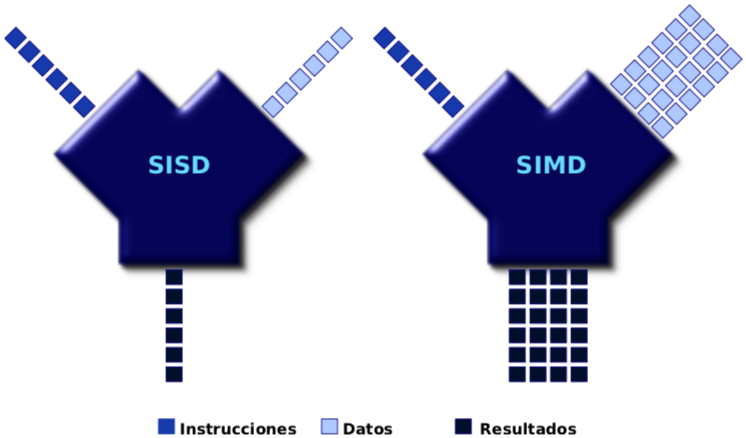
\includegraphics[width=0.45\textwidth]{imagenes/sisdsimd.png} &
    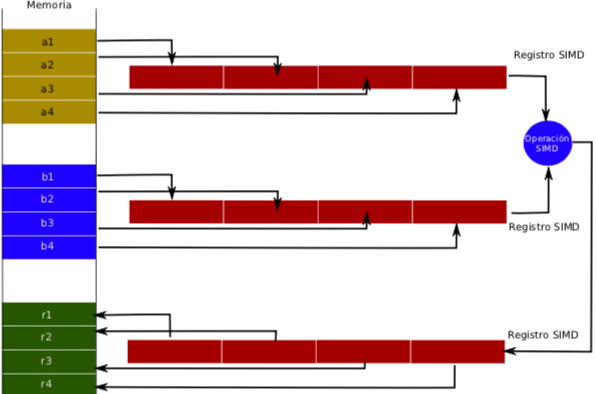
\includegraphics[width=0.45\textwidth]{imagenes/registrossimd.png}\\
  \end{tabular}
 \end{center}

\subsection{Objetivos Generales}
Además de la exploración del modelo SIMD se repasaron conceptos y técnicas de programación vectorizada en C y ASM dentro del campo de aplicación del procesamiento de imagenes. Para esto se llevó a cabo la implementación de los siguientes filtros para imágenes:

\begin{center}
 \begin{tabular}{cccc}
   
\includegraphics[width=0.2\textwidth]{imagenes/island.png} &
   
\includegraphics[width=0.2\textwidth]{imagenes/island-blit.png} &
   
\includegraphics[width=0.2\textwidth]{imagenes/island-monocromatizar.png} \\
   Imagen original & Blit & Monocromatizar \\
   \\
   
\includegraphics[width=0.2\textwidth]{imagenes/island-ondas.png} &
   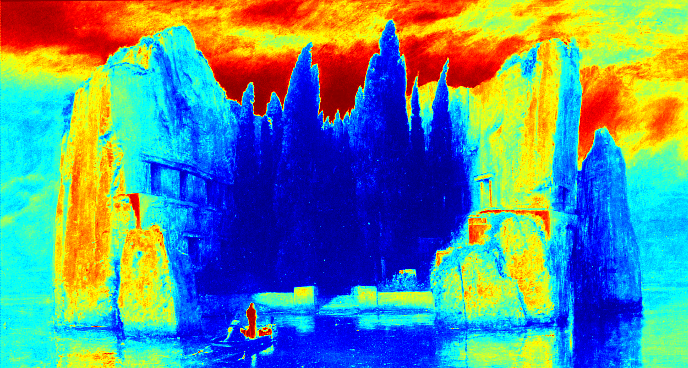
\includegraphics[width=0.2\textwidth]{imagenes/island-temperature.png} &
   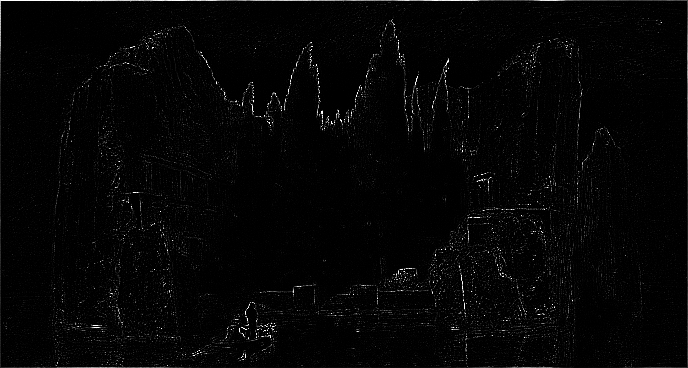
\includegraphics[width=0.2\textwidth]{imagenes/island-edge.png} \\
   Ondas & Temperature & Edge \\
 \end{tabular}
\end{center}

\subsection{Metodología}
La elaboración del trabajo se dividió en dos etapas. En primer lugar, se implementaron ambos filtros tanto en lenguaje C como en lenguaje ensamblador para la arquitectura x86-64 de Intel. En este último caso, se utilizaron las instrucciones SSE de dicha arquitectura, que aprovechan el ya mencionado modelo SIMD para procesar datos en forma paralela.

Una vez realizadas estas implementaciones, fueron sometidas a un proceso de comparación para extraer conclusiones acerca de su rendimiento. Con este fin, se experimentó con variaciones tanto en los datos de entrada como en detalles implementativos de los mismos algoritmos. De esta manera, se pudo recopilar datos sobre el comportamiento de cada implementación, y contrastar estos resultados con diversas hipótesis previamente elaboradas.

Para las mediciones se corrieron los algoritmos en una computadora con las siguientes especificaciones:

\begin{center}
  \begin{tabular}{cccc}
    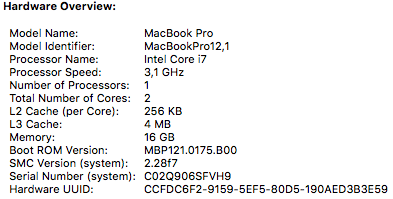
\includegraphics[width=0.5\textwidth]{imagenes/hardware.png} &
    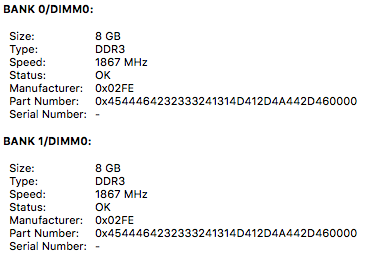
\includegraphics[width=0.5\textwidth]{imagenes/memory.png} \\
  \end{tabular}
 \end{center}

 Asimismo se utilizó la siguiente combinación de sistema operativo y compiladores: Ubuntu/Xenial64 16.04.4 LTS, GCC versión 5.4.0 y NASM versión 2.11.08. Para compilar el código C se usaron los flags \textit{-ggdb -Wall -Wno-unused-parameter -Wextra -std=c99 -pedantic -m64 -O3} y para ASM \textit{-felf64 -g -F dwarf} conforme a los archivos proporcionados por la cátedra de la materia.


A continuación introducimos los filtros y sus respectivas implementaciones, luego describimos los tests realizados y los resultados obtenidos, y finalmente a partir de estos datos otorgamos algunas conclusiones sobre la experiencia realizada.